\subsection{Uso de imágenes sintéticas}

	En esta sección se busca ver el impacto producido por las imágenes sintéticas en la clasificación. Es decir, se buscar entrenar al clasificador con dos grupos de imágenes. El primer conjunto está conformado por imágenes sintéticas alteradas cuyo proceso de creación fue detallado en la sección \ref{subsection:impl_propia}. El segundo esta conformado por una combinación del primer grupo con el conjunto de imágenes reales usado en \ref{subsection:baseline}.
	
	El grupo de imágenes de fuentes sintéticas de computadora que se usa para crear los caracteres sintéticos fue extraído del dataset mencionado en \ref{subsection:evaluacion} y consiste en 1000 imágenes por clase. De este conjunto se crearon 6 variaciones diferentes, con el objetivo de observar el impacto que tiene la cantidad de caracteres sintéticos al momento de clasificar imágenes de caracteres naturales. La cantidad de muestras por clase (variaciones) en cada conjunto de entrenamiento es la siguiente:
	\begin{itemize}
		\item Muestras por clase : $ mpc \in \{ 50,100,250,500,1000,2000\}$
	\end{itemize}
	
	Estas variaciones son puestas a prueba en el primer experimento de la sección.
	
	El segundo conjunto de imágenes sintéticas se creó con la finalidad de observar el impacto en la clasificación de integrar, en diferentes proporciones, imágenes sintéticas y reales al conjunto de entrenamiento. Dada la escasa cantidad de imágenes naturales para el entrenamiento (15 en total por cada clase), se busca complementar esto integrando datos sintéticos. Por consiguiente, se decide crear 9 conjuntos de entrenamiento donde en cada uno se incorporan diferentes proporciones de imágenes sintéticas a las 15 reales existentes. La proporción de cada conjunto de entrenamiento es: 
	
	$$(15, x)~\textit{con}~ x \in \{0,3,8,15,30,75,150,300,750,1500 \}$$
	
	El primer elemento de la tupla $(15, x)$ corresponde a la cantidad de imágenes reales, cuyo valor es fijo. El segundo elemento de la tupla hace referencia a la proporción de caracteres sintéticos. Es fácil observar que a medida que aumentamos la proporción, la cantidad de caracteres naturales se va volviendo cada vez más despreciable. El hecho de no considerar imágenes sintéticas inicialmente $(15,0)$ tiene como finalidad el observar el cambio que se produce desde el inicio cuando no hay caracteres sintéticos en el entrenamiento.
	
	Este segundo grupo de imágenes es puesto a prueba en el último experimento de la sección.

	Los parámetros utilizados durante la creación de las imágenes sintéticas son, como se explicó en \ref{subsection:impl_propia}, escala, rotación, transvección, traslación, blur y ruido Gaussiano. Dado que hay un abanico bastante grande de valores para asignarles a estas transformaciones, se decidió por asignarle a cada una un rango de valores razonable. Dado que los autores en \cite{wang} no especifican el rango de valores para las transformaciones que utilizan, se procedió a establecer los siguientes intervalos para todas las transformaciones utilizadas:
	
	\begin{itemize}
		\item Transvección: $n \in [-0.20 ; 0.20]$
		\item Suavizado gaussiano (blur): $\sigma \in [0 ; 2]$
		\item Escala: $a=d \in [0.8; 1.25]$
		\item Rotación (en radianes): $\theta \in (-0.1; 0.1)$
		\item Ruido Gaussiano: $\sigma \in [1; 30]$
	\end{itemize}

\subsubsection{Primer Experimento: Conjunto de imágenes sintéticas}
\label{subsubsection:primer-experimento}

	En el primer experimento, se procederán a mostrar los resultados obtenidos de haber utilizado el primer conjunto de imágenes. Los gráficos van a representar la relación entre la cantidad de imágenes sintéticas por clase (dado por \textit{IPC} en las siguientes figuras) y la precisión de clasificación dada por los $4$ valores a evaluar que son las dimensiones de los grupos. Teniendo en cuenta los resultados anteriores con las imágenes reales, se decidió por trabajar con la mejor configuración encontrada salvo por el parámetro \textit{B/G}(\textit{bits por grupo}). Este último parámetro se mantuvo con el fin de seguir evaluándolo con estos nuevos experimentos.
	
	El baseline con el que se comparan los resultados es el obtenido en \ref{subsection:baseline} para las imágenes sintéticas cuyo valor es $0.43$.

			\begin{figure}[htbp]
				\centering
				\centerline{
					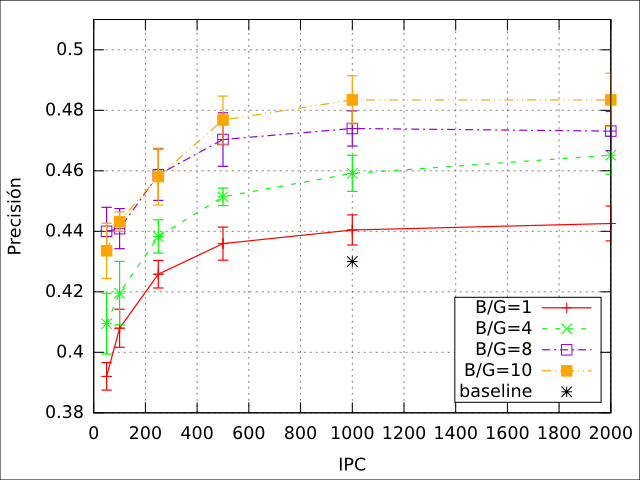
\includegraphics[scale=0.5]{img/resultados/sinteticas/mean_2040.png}
				}
				\caption[Sintéticas media 2040]{El gráfico muestra los resultados obtenidos de haber utilizado la mejor configuración analizada y haciendo uso de vectores binarizados de longitud $2040$.}
				\label{fig: Sinteticas-media-2040}
			\end{figure}

	En cuanto a los experimentos con imágenes sintéticas, basándonos en los resultados plasmados en la figura \ref{fig: Sinteticas-media-2040}, es interesante observar que a medida que agregamos más imágenes sintéticas por clase, aumenta la performance del clasificador en todos los casos. Inicialmente, el crecimiento es más pronunciado hasta llegar a un punto (a partir de las 1000 IPC) en donde el mismo no es tan notable y en algunos casos tiende a ``aplanarse''. En base a esto, no tiene sentido trabajar con más de $1000$ imágenes por clase, pues computacionalmente es más costoso y no se obtiene una precisión que justifique su uso. En el mejor de los casos, al usar grupos de $10$ bits, la diferencia en performance entre usar $1000$ ó $2000$ imágenes por clase es nula. El hecho de que se hayan necesitado $2000$ muestras por clase para alcanzar una performance cercana al $49\%$, también refleja que las imágenes sintéticas no aportan la misma cantidad de información que las reales.
	
	Una particularidad de este experimento con respecto a los anteriores (ver \ref{subsubsection: eval_esquemas}), es que los mejores resultados se obtienen cuando la cantidad de bit por grupo (dado por \textit{B/G} en \ref{fig: Sinteticas-media-2040}) es grande. Esta tendencia se ve en todos los niveles a medida que aumenta \textit{IPC}.

	Por último, en cuanto a la comparación con el baseline, los resultados en la mayoría de los casos son superiores incluso habiendo entrenado al clasificador con menos imágenes por clase ($\leq 1000$). Por lo tanto, se puede decir que la configuración elegida hace un mejor uso de los datos de entrenamiento.
	
\subsubsection{Segundo Experimento: Conjunto de imágenes mixto}
	
	En este último experimento, se van a mostrar los resultados correspondientes de haber entrenado al clasificador \textit{Random Ferns} con conjuntos de entrenamiento mixtos. Se procederá a mostrar la figura con la mejor configuración. También se mostrarán las matrices de confusión para este caso. Al igual que en \ref{subsubsection:primer-experimento}, se va a utilizar la mejor configuración obtenida en \ref{subsection:baseline} descartando también al parámetro $B/G$.

	El gráfico a continuación presenta el eje \textit{x} en escala logarítmica para poder apreciar mejor las variaciones que se dan al experimentar con valores cercanos entre sí.

			\begin{figure}[!htbp]
				\centering
				\centerline{
					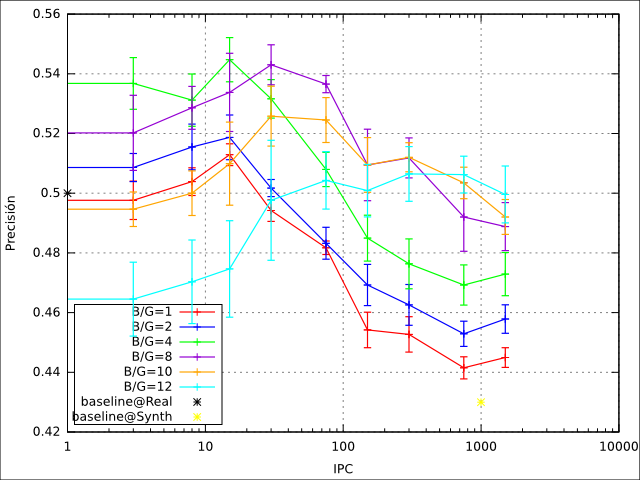
\includegraphics[scale=0.6]{img/resultados/mixtas/best_mean_2040.png}
				}
				\caption[Mixtas media mejor resultado]{El gráfico muestra la configuración que devolvió los mejores resultados.}
				\label{fig: Mixtas-media-mejor}
			\end{figure}

	De la figura \ref{fig: Mixtas-media-mejor} se puede desprender el siguiente análisis. El primero, y uno de los más importantes, hace referencia a la influencia en la clasificación de ir agregando de manera incremental imágenes sintéticas durante la etapa de entrenamiento. Se puede observar que a nivel general todos los experimentos llegaron a un punto donde su performance se desplomó al seguir agregando imágenes. Sin embargo, este cambio ocurrió en diferentes momentos dependiendo del caso. Por ejemplo, cuando trabajamos con grupos de dimensionalidad baja ($1$ y $4$ bits por grupo), la precisión del clasificador va en aumento hasta que se llega a un máximo correspondiente al haber entrenado al sistema con igual cantidad de imágenes reales y sintéticas. A partir de ese punto, el seguir incrementando la proporción de sintéticas sobre reales trajo efectos negativos en los resultados como se puede apreciar en el gráfico presentado. En los casos donde consideramos $10$ bits por grupo el rendimiento se desploma cuando consideramos más de 75 imágenes sintéticas. Cuando superamos esa proporción se puede ver que la performance decae. Todo esto se debe a que llegado cierto punto, el clasificador aprende las particularidades de los datos sintéticos. Es decir, a medida que la cantidad de imágenes sintéticas supera en gran proporción a la imágenes reales, la información almacenada sobre las primeras adquiere más relevancia en la clasificación haciendo que la performance disminuya.

	 La mejor curva en el gráfico la obtenemos cuando consideramos $4$ bits por grupo y entrenamos al clasificador con la misma cantidad de imágenes sintéticas que reales. Este resultado coincide respecto al análisis realizado para los experimentos con imágenes reales donde consideramos que el mejor parámetro era considerar grupos de $4$ bits. En la mayoría de los casos se dan buenos resultados cuando la cantidad de imágenes sintéticas sobre las reales es la misma ($1$ y $4$) o se duplica ($8$ y $10$).

	 Teniendo en cuenta los baselines presentados en la tabla \ref{table: Baseline-Table} y el hecho de que estos experimentos tienen una base inicial de imágenes reales, se puede observar que el baseline ``SYNTH'' es superado. En cuanto al baseline ``NATIVE'', a diferencia de los resultados obtenidos con las imágenes reales (que se pueden ver en el inicio de cada curva de la figura \ref{fig: Mixtas-media-mejor}), el incremento en la precisión del clasificador no es muy notorio; sin embargo, el hecho de poder incrementar la performance haciendo uso de imágenes sintéticas es un avance. Llama la atención que el usar la misma cantidad de imágenes reales y sintéticas no haya producido un incremento más marcado en la performance. Sin embargo, como pudimos ver en \ref{fig: Sinteticas-media-2040}, ni con 50 imágenes sintéticas por clase se podía alcanzar un valor similar al del baseline.

	Otro de los análisis realizado en el trabajo pasa por los errores de clasificación que se han observado. En las figuras \ref{fig: Mixtas-Matrix-media-mejor} y \ref{fig: MatrizIns-Mixtas-media-mejor}, se pueden ver dos matrices de confusión. La primer corresponde al mejor resultado obtenido en la figura \ref{fig: Mixtas-media-mejor} y la segunda es una versión de la primera donde no diferenciamos caracteres mayúsculas de minúsculas.

	En la región central, dada por la diagonal de la matriz, se encuentran las muestras que fueron bien clasificadas durante la evaluación del clasificador. Existen zonas dentro de la diagonal que corresponden a clases que obtuvieron una tasa de acierto inferior al $30\%$ (los cuadrados en escala de azul dentro de la imagen). En estas clases son más comunes los siguientes errores:

	\begin{itemize}
		\item No poder distinguir mayúsculas de minúsculas para los caracteres involucrados. En la figura \ref{fig: Error-CaseSensitive} se puede observar un ejemplo donde, incluso para las personas, es difícil notar la diferencia.
		\item Confundir un carácter por otro similar. La figura \ref{fig: Error-Apariencia} muestra varios ejemplos donde se pueden confundir caracteres.
	\end{itemize}

		\begin{figure}[htbp]
			\centering
			\subfloat[c minúscula\label{fig: Lower-case-c}]{
				\fbox{ 
\includegraphics[scale=1]{img/errores_clasif/CaseSensitiveError/lowerCase_c.png} }
			}
			\subfloat[C mayúscula\label{fig: Upper-case-C}]{
				\fbox{ 
\includegraphics[scale=1]{img/errores_clasif/CaseSensitiveError/upperCase_C.png} }
			}
			\subfloat[z minúscula\label{fig: Lower-case-z}]{
				\fbox{
\includegraphics[scale=1]{img/errores_clasif/CaseSensitiveError/lowerCase_z.png} }
			}
			\subfloat[Z mayúscula\label{fig: Upper-case-Z}]{
				\fbox{ 
\includegraphics[scale=1]{img/errores_clasif/CaseSensitiveError/upperCase_Z.png} }
			}
			\\
			\subfloat[x minúscula\label{fig: Lower-case-x}]{
				\fbox{ 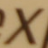
\includegraphics[scale=1]{img/errores_clasif/CaseSensitiveError/lowerCase_x.png} }
			}
			\subfloat[X mayúscula\label{fig: Upper-case-X}]{
				\fbox{ 
\includegraphics[scale=1]{img/errores_clasif/CaseSensitiveError/upperCase_X.png} }
			}
			\subfloat[v minúscula\label{fig: Lower-case-v}]{
				\fbox{ 
\includegraphics[scale=1]{img/errores_clasif/CaseSensitiveError/lowerCase_v.png} }
			}
			\subfloat[V mayúscula\label{fig: Upper-case-V}]{
				\fbox{ 
\includegraphics[scale=1]{img/errores_clasif/CaseSensitiveError/upperCase_V.png} }
			}
			\caption[Error entre mayúscula y minúscula]{Error de clasificación donde se confunde el carácter en mayúscula y en minúscula.}
			\label{fig: Error-CaseSensitive}
		\end{figure}

		\begin{figure}[htbp]
			\centering
			\subfloat[o minúscula\label{fig: Lower-case-o}]{
				\fbox{ 
\includegraphics[scale=1]{img/errores_clasif/ShapeError/lowerCase_o.png} }
			}
			\subfloat[O mayúscula\label{fig: Upper-case-O}]{
				\fbox{ 
\includegraphics[scale=1]{img/errores_clasif/ShapeError/upperCase_O.png} }
			}
			\subfloat[número 0\label{fig: Number-0}]{
				\fbox{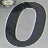
\includegraphics[scale=1]{img/errores_clasif/ShapeError/number_0.png} }
			}
			\\
			\subfloat[I mayúscula\label{fig: Upper-case-I}]{
				\fbox{ 
\includegraphics[scale=1]{img/errores_clasif/ShapeError/upperCase_I.png} }
			}
			\subfloat[l minúscula\label{fig: Lower-case-l}]{
				\fbox{ 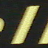
\includegraphics[scale=1]{img/errores_clasif/ShapeError/lowerCase_l.png} }
			}
			\subfloat[número 1\label{fig: Number-1}]{
				\fbox{ 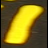
\includegraphics[scale=1]{img/errores_clasif/ShapeError/number_1.png} }
			}
			\caption[Error de apariencia]{Error de apariencia entre caracteres.}
			\label{fig: Error-Apariencia}
		\end{figure}


	El no poder distinguir mayúsculas de minúsculas se ve reflejado en la matriz \ref{fig: MatrizIns-Mixtas-media-mejor} en dos regiones. Dichas regiones corresponden a dos submatrices, la primera ubicada en la esquina inferior izquierda y la segunda en la esquina superior derecha. Ambas submatrices, no involucran los caracteres numéricos y se puede ver en la diagonal de cada una, la cantidad de imágenes de cada clase donde se confundió la versión mayúscula y minúscula. Es muy difícil, incluso para las personas, clasificar imágenes de caracteres recortados donde no hay una clara distinción entre la versión mayúscula y minúscula.

	Los errores de ``apariencia'' como los expuesto en la figura \ref{fig: Error-Apariencia} están distribuidos por toda la matriz, habiendo casos donde la similitud es evidente y en otros casos más raros donde no existe directamente. Este último caso, donde no existe similitud, puede solventarse si se entrenase al clasificador con más imágenes.

	La matriz \ref{fig: MatrizIns-Mixtas-media-mejor} se creó con el objetivo de reflejar otra punto de vista de los resultados, donde no se consideren los caracteres en mayúscula. Se puede observar que la diagonal de la matriz mejora con respecto a la anterior y además se acentúan aún más los problemas de apariencia que surgen entre ciertos caracteres. Por ejemplo, los errores de clasificación en el carácter ``i'' que se confunde con una ``l'' en muchos casos, o el carácter ``o'' con el número ``0''. La mayoría de los errores de clasificación se podrían corregir si las imágenes de los caracteres sintéticos pudieran almacenar el mismo nivel de información que una imagen real. Esta diferencia se pudo observar en los resultados pues, el conjunto de imágenes sintéticas en este trabajo no pudo superar en precisión al conjunto de imágenes reales.

			\begin{figure}[!htbp]
				\centerline{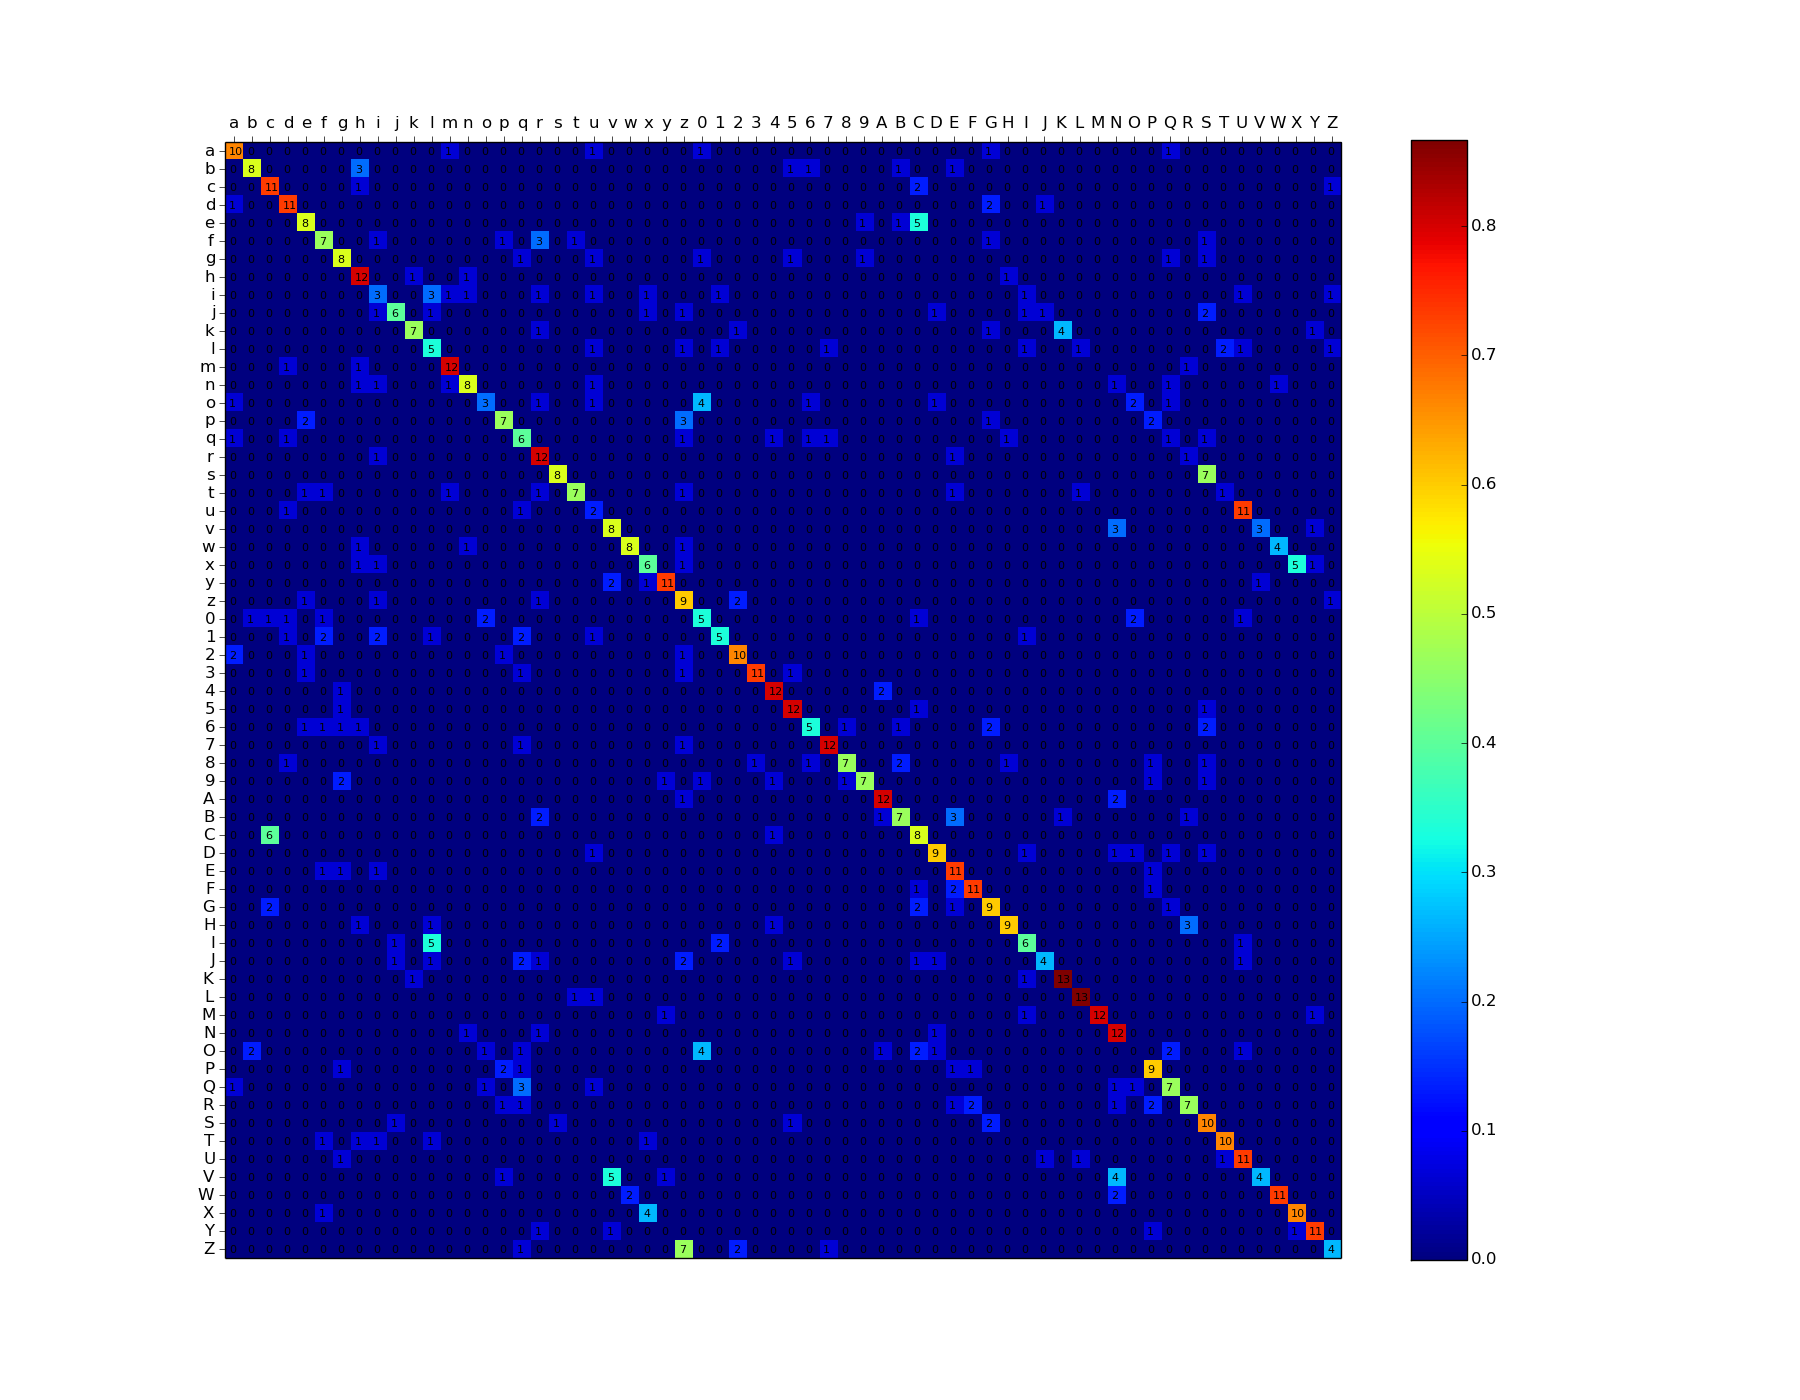
\includegraphics[scale=0.4]{img/resultados/mixtas/best_mean_matrix_Alpha0,01_2040-4.png}}
				\caption[Mixtas Matriz expon]{Matriz de correlación del gráfico \ref{fig: Mixtas-media-mejor} para el mejor resultado.}
				\label{fig: Mixtas-Matrix-media-mejor}
			\end{figure}

			\begin{figure}[!htbp]
				\centerline{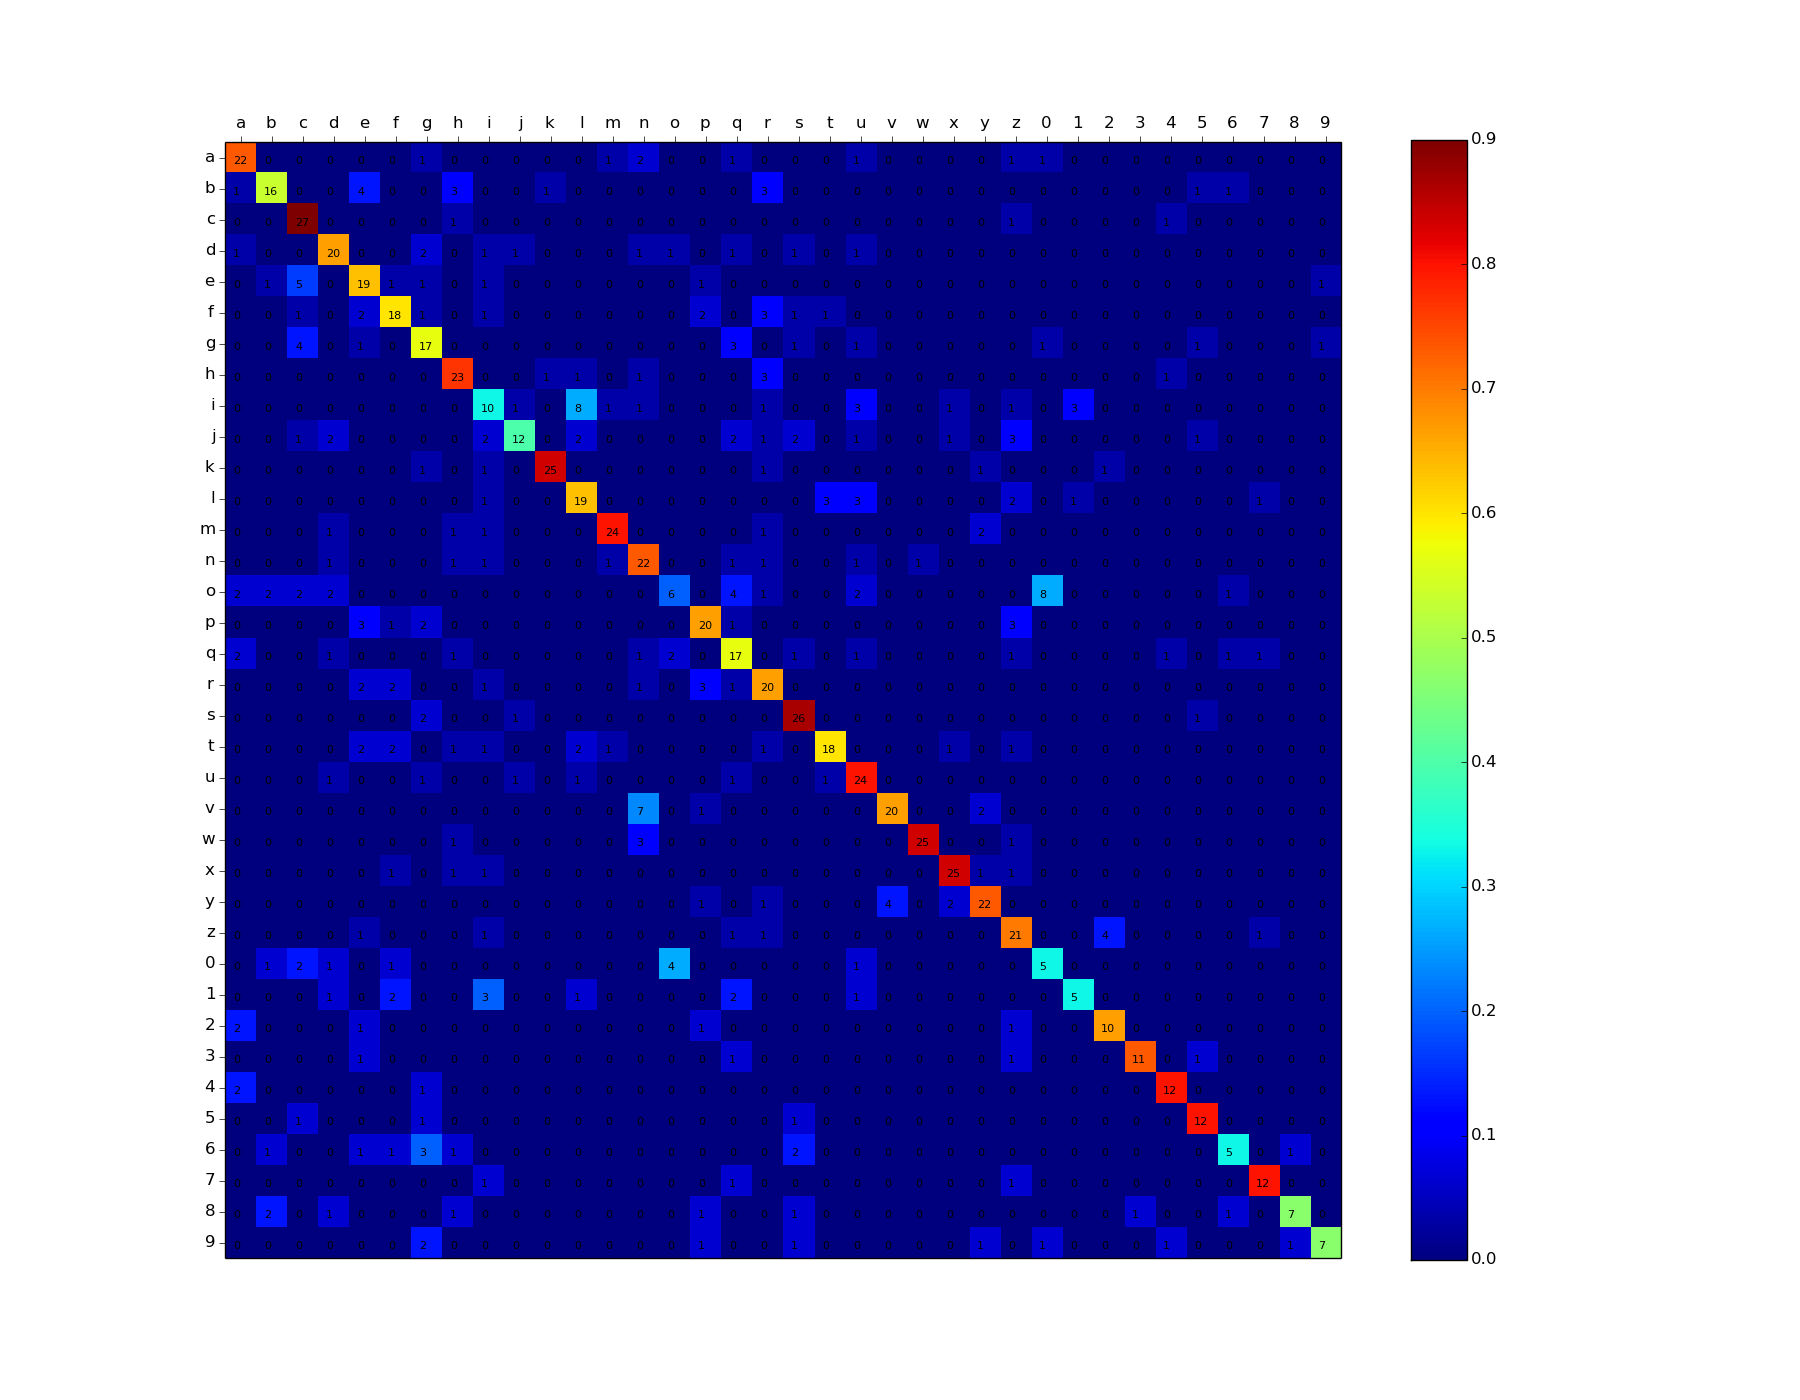
\includegraphics[scale=0.4]{img/resultados/mixtas/best_mean_matrix_Alpha0,01_2040-4_ins.png}}
				\caption[Matriz de correlación ``case insensitive'' para mixtas media]{Matriz de correlación del gráfico \ref{fig: Mixtas-media-mejor} para el mejor resultado no teniendo en cuenta los caracteres en mayúscula.}
				\label{fig: MatrizIns-Mixtas-media-mejor}
			\end{figure}
